\problemname{Car Vet} Bob Roberts is the self proclaimed ``Car Vet'' who owns
several junk car lots where people can come and search for spare parts for
their (ailing) cars. The cars in each lot are parked in a fenced-in $m \times
n$ grid lot, where each car takes up two grid squares. Each lot also has zero or
more grid locations devoted to piles of parts (fenders, $8$-track tape players,
wheel covers, fuzzy dice, etc.); these locations are effectively blocked.
Business has been so good that each of Bob's lots has only one empty grid
space left.

From time to time, Bob or one of his lot attendants drops a part on the ground
and it rolls underneath one of the cars.
The only way to retrieve it is to move the car out of the way. 
Depending on the location of the empty grid space, it may be necessary to move
several cars in order to achieve this. Cars can only move forward or backward,
and car movement is also constrained by the fence, which prevents any
car from moving off the lot, and by the blocked grid locations containing
piles of parts.

Figure \ref{fig:sample1} shows an example. An ambihelical hexnut has rolled
under car number $3$ in row $3$, column $3$ of the grid (shaded dark gray).
The space in row $1$, column
$3$ is empty and the space in row $3$, column $4$ is blocked. The only way to 
retrieve the part is to move car $8$, then car $4$, then car $3$. Note that if the
locations of the empty grid cell and the blocked grid cell were reversed,
it would not be possible to retrieve the part.

\begin{figure}[!h]
\centering
%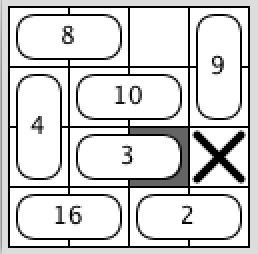
\includegraphics[scale=1.0]{sampleinput1.png}
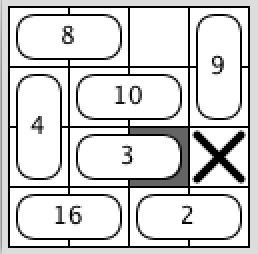
\includegraphics[width=.25\linewidth]{sampleinput1.png}
\caption{Sample lot. Cars $8$, $4$, and $3$ must be moved, in that order, to
uncover the grid location in row $3$, column $3$. This corresponds to Sample
Input $1$.}
\label{fig:sample1}
\end{figure}

The problem here should be obvious: For a given location
Bob would
like to know how to move cars around to uncover that location, or
if it is even possible to uncover it.

\section*{Input} Input starts with a line containing two positive integers $m$
$n$ $(m, n \leq 250)$ indicating number of rows and columns
of the junk car lot. Following this are
$m$ lines each containing $n$ integers; the $j^{th}$ value on the $i^{th}$ line
indicates the contents of the grid square at row $i$, column $j$.
All values $v$ are in the range $-2 \leq v \leq 62\,500$.
Each non-negative value indicates that half of a junk car is in that location.
Every non-negative
value appears exactly twice and these two occurrences
are horizontally or vertically adjacent to each other.
A value of $-1$ indicates the empty grid location and a value of
$-2$ indicates a blocked location.
There is always exactly one empty location and
at least one car, but
there may be zero or more blocked locations.
Following these $m$ lines is a single line containing two
integers $r$ $c$ $(1 \leq r,c \leq 250)$ indicating the row and column number of the
desired location to be uncovered. This
will always correspond to the location of a junk car.

\section*{Output} Display, on a single line separated by spaces, the numbers
of the cars that
must be moved to make the given location empty. They should appear in the
order in which they must be moved.  If there is
more than one sequence of possible moves, display the sequence of shortest
length. If there is still a tie, display the sequence that comes
lexicographically first according to the car numbers in the sequence.
If it is not possible to
uncover the desired location, display {\tt impossible}. 
